\chapter{MoVe\_IT kc705 Tera10 firmware update}
\section{Introduction}
\noindent As explained in the previous chapters a good VHDL design, in order to improve readability and order, uses separate modules for each main task of the firmware. Each module is connected with wires (signals) to the others. The first half of this chapter will analyze the structure of the kc705 tera10 firmware, while the second half will be focused on the thesis work; this comprehends the HDL additions to the firmware, the software simulations and the test simulations on chip.
In section \ref{hardware} will be described a simple level translator built for simulation purposes while in sections \ref{testbench} and \ref{testboard} will be briefly analyzed the experimental setup.

\section{Firmware structure}
\noindent
\begin{figure}[H]
	\centering
	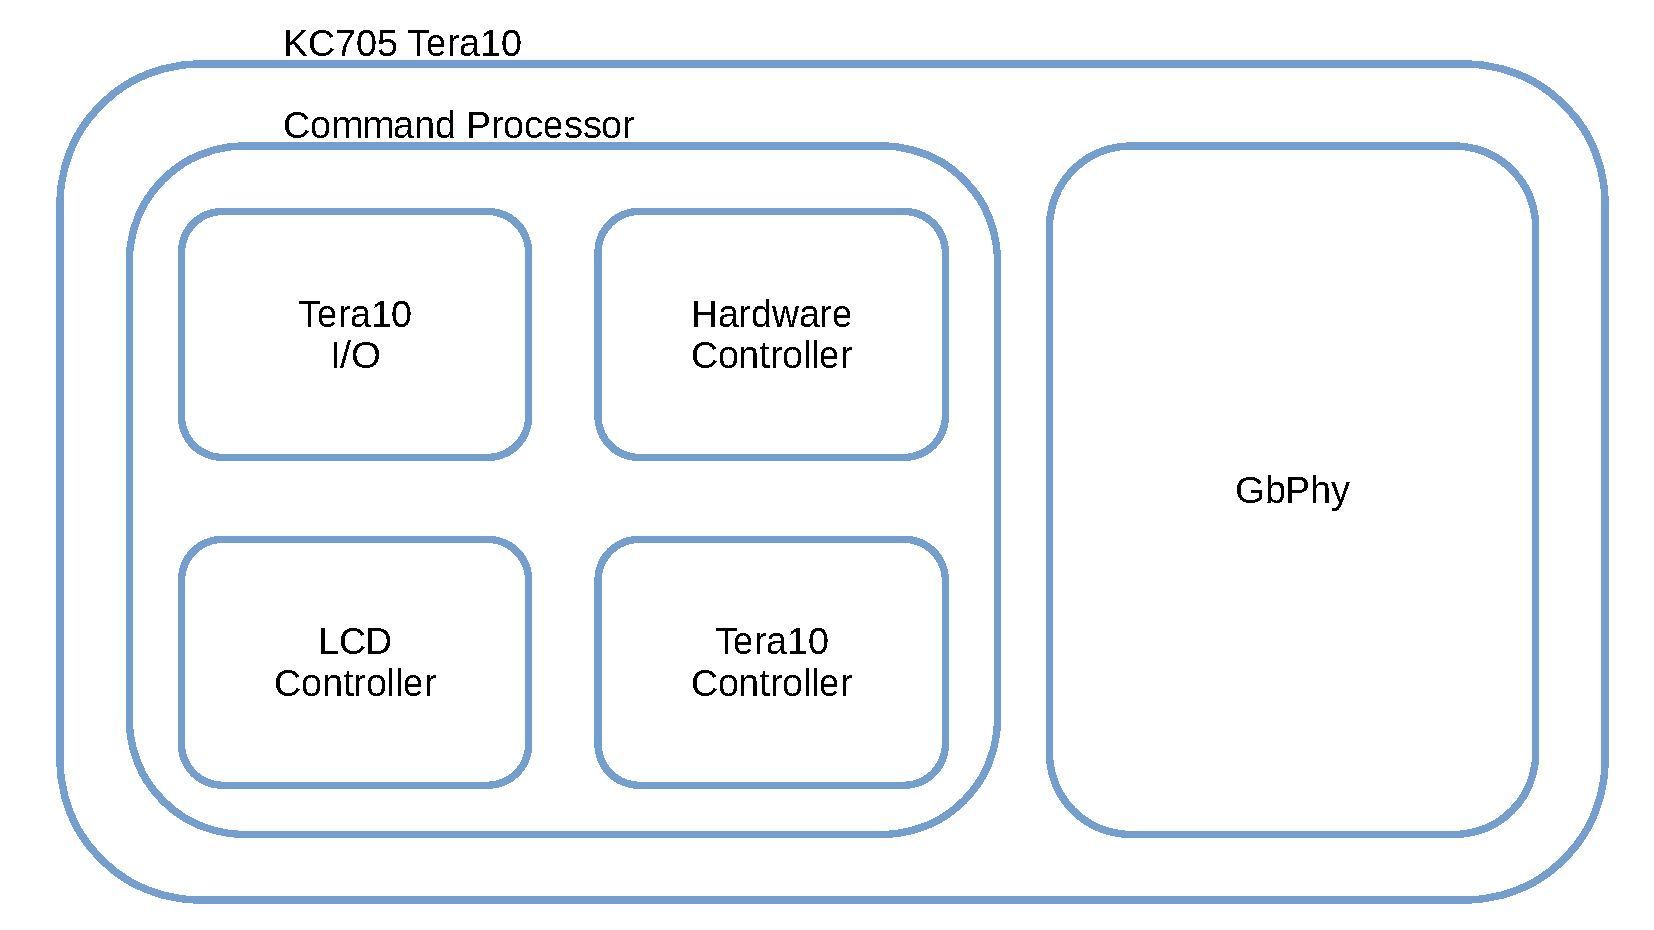
\includegraphics[width=0.7\linewidth]{IMG/ch4/TERA10}
	\caption{KC705 tera10 firmware structure}
	\label{fig:tera10}
\end{figure}
\begin{itemize}
	\item \textbf{KC705 TERA10}: this is the main module, everything lives inside it, thus it contains no logic, only component declarations and port-maps. In this module can be set the firmware version ("B20C" for example) that will the displayed on the LCD.
	%%%%%%%%%%%%%%%%%%%%%%%%%%%%%%%%%%%%%%%%%%%%%%%%%%%%%%%%%%%%%%%%%%%%%%%%%%
	\item \textbf{GbPhy}: the communication between FPGA and computer is done via Ethernet cable using a UDP (User Datagram Protocol). This is done via firmware and also thanks to a dedicated chip connected on the board to the RJ45 connector called "PHY".
	\newline
	PHY is an abbreviation for "physical layer" and is an electronic circuit, usually implemented as a chip (integrated circuit) mandatory to implement links between physical mediums such as copper or optical fiber. It basically converts data between a "clean" clocked digital stream form that is suitable only for very short distance communication (centimetres) and an analog form that is suitable for long range transmission (meters or more).
	The chip on the KC705 board is able to transmit data up to 1Gb/s.
	\newline
	The PHY is thus firmware controlled, in the MoVe\_IT project the reception and sending of messages is managed by another project of the Turin INFN group called GbPhy. This thesis will  not focus on how it works, but only on its main characteristics\cite{gbphy}.     
	\begin{figure}[H]
		\centering
		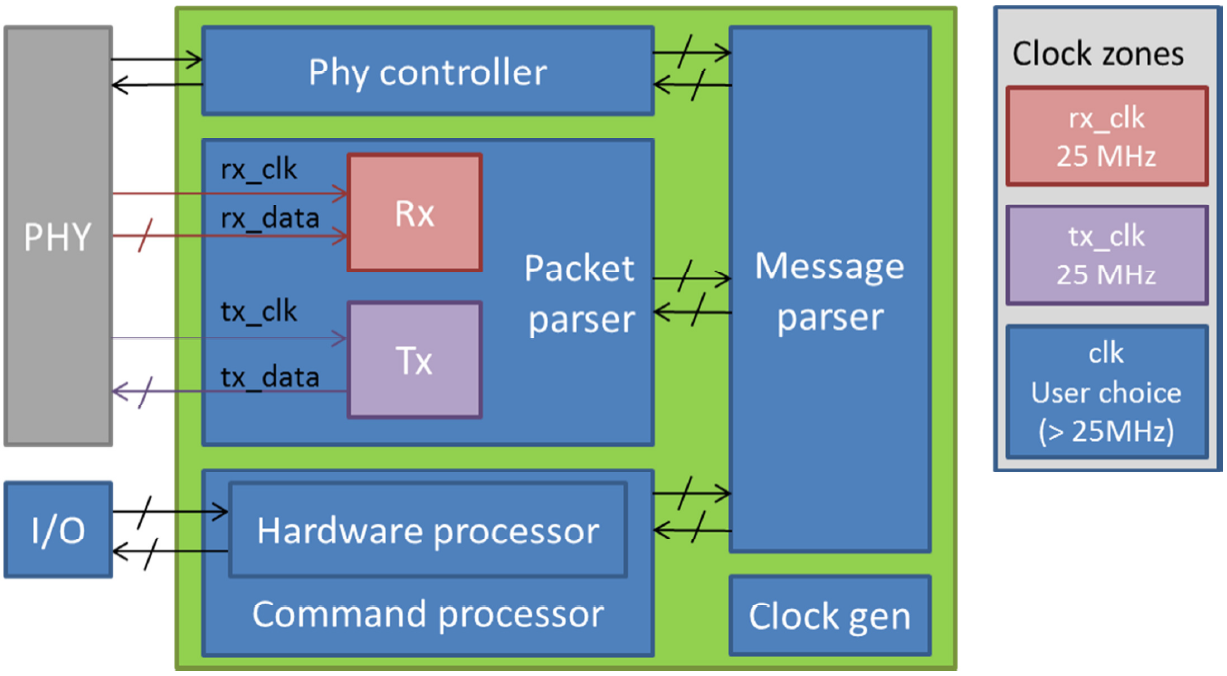
\includegraphics[width=0.7\linewidth]{IMG/ch4/PHY100}
		\caption{GbPhy firmware structure}
		\label{fig:phy100}
	\end{figure}
	\noindent GbPhy provides a UDP-based Ethernet control link based on a fixed length 8 byte protocol.
	For each 8 byte message the user can send 4 bytes of data. The data is thus divides as follow:
	\begin{itemize}
		\item command\_contents(31 downto 28) => sub-system target;
		\newline
		For this application this can be x"1" for hardware commands, x"2" for LCD commands and x"4" for Tera10 commands.
		\item command\_contents(27 downto 20) => sub-system command id;
		\newline
		Each task (or command) has an id, a name with which it can be called, an example of this is the list of commands in the \textit{Tera10 Controller} part in the next pages.
		\item command\_contents(19 downto 0) => sub-system command data;
		\newline
		This 20 bits are the data that may be needed to the firmware; for example, this can be the value of a DAC that needs to be set, or it can be a list of channels that the user wants to enable or it can also be the value of a counter that the user want to read. 
	\end{itemize} 
	%%%%%%%%%%%%%%%%%%%%%%%%%%%%%%%%%%%%%%%%%%%%%%%%%%%%%%%%%%%%%%%%%%%%%%%%%% 
	\item \textbf{Command Processor}: this module is mainly a wrapper for every module that will be presented from now on. It also 
	redirects the commands in accord with the sub-system target.
	%%%%%%%%%%%%%%%%%%%%%%%%%%%%%%%%%%%%%%%%%%%%%%%%%%%%%%%%%%%%%%%%%%%%%%%%%%
	\item \textbf{LCD Controller}: it is the module that drives the 16x2 LCD display of the board.
	\begin{figure}[H]
		\centering
		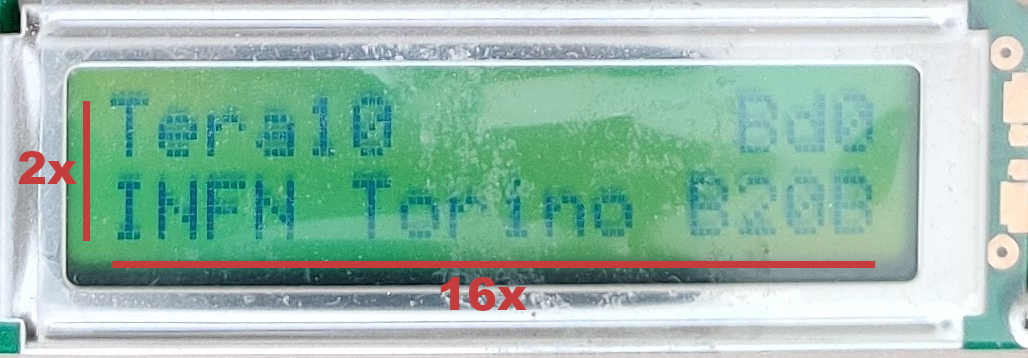
\includegraphics[width=0.5\linewidth]{IMG/ch4/LCD}
		\caption{KC705 tera10 LCD output}
		\label{fig:lcd}
	\end{figure}
	\noindent This module contains multiple processes, FSMs (Finite State Machines) and a RAM module. The first FSM manages the start-up sequence for the LCD, the second does the conversion of the firmware version from hex to ASCII, a third one sends one by one the characters to the display while a fourth one manages the communications with the UDP module. In fact the firmware can not only display a fixed pre-selected banner, but also a user-sent 'message' from the pc.
	The LCD is extremely useful when working with more than one card for discriminating one from another and for keeping track of the firmware version of each board.
	%%%%%%%%%%%%%%%%%%%%%%%%%%%%%%%%%%%%%%%%%%%%%%%%%%%%%%%%%%%%%%%%%%%%%%%%%%    
	\item \textbf{Tera10 I/O}: this module contains the declaration and port-map for 24 \textit{tera10 channel coincidence} modules\cite{limardi}; each module receives as an input the data from two channels of the ABACUS2 chip, this signal is thus de-serialized with a 1GHz frequency (\textit{serdes\_clk}), ten times higher than the main clock (100MHz). The output of the de-serializer is a 10 bit bus (one for each signal) to which it is added, using a shift register, the last bit from the previous bus. This is done in order to not lose any transition (high/low) from one packet and the next one.
	\newline
	The counting of the number of pulses is done with a LUT (Look Up Table) that from a 11bit bus gives back a 3bit logic vector corresponding to the number from 0 to 1. This result is used to update a 32bit counter for each channel; in figure \ref{fig:coincidence} those are N1 for ch0 and N2 for ch1.
	\newline
	In order to count with efficiency even at high rates a previous student implemented in the firmware pile-up correction algorithms. AND and OR logic combinations between the two channels 10bit bus are done, compared with others LUTs and added to four new 32bit counters ($N_{AND}$, $T_{AND}$, $N_{OR}$ and $T_{OR}$). 
	\begin{figure}[H]
		\centering
		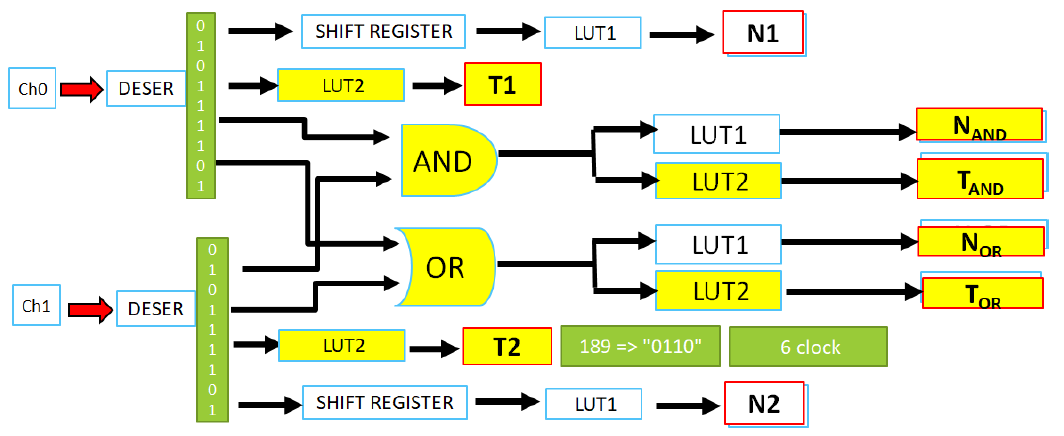
\includegraphics[width=0.7\linewidth]{IMG/ch4/COINCIDENCE}
		\caption{KC705 tera10 channel coincidence architecture diagram}
		\label{fig:coincidence}
	\end{figure}
	\noindent The counters $T_{1}$, $T_{2}$, $T_{AND}$ and $T_{OR}$ contain the number of clock strokes in which one of the two channel or a logic combination of both is \textit{high}.
	%%%%%%%%%%%%%%%%%%%%%%%%%%%%%%%%%%%%%%%%%%%%%%%%%%%%%%%%%%%%%%%%%%%%%%%%%% 
	\item \textbf{Tera10 Controller}: this module is strictly connected to the previous one (\textit{Tera10 I/O}), in fact it receives every counter from the previous block and manages the data in accord to the commands sent by the user. Some of the more used and important commands are:
	\begin{itemize}
		\item x"01" \textit{reset serdes}: send reset signal for the de-serializer.
		\item x"02" \textit{reset counters}: every counter for each \textit{tera10 channel coincidence} module is set to 0.
		\item x"10" \textit{set counter enable}: to enable selected counters. This is done by dividing the channels in blocks of 16. When a 20bit data command is sent bits 18-17-16 are used to identify the block, and the next 16bit are encoded one-hot for each channel; for example, to enable channel 2 the data to be sent is \textit{0-000-0000000000000010} and to enable channel 18 the data is \textit{0-001-0000000000000100}.   
		\item x"11" \textit{read counter}: read selected counter; the firmware response is a 16bit bus, thus 2 commands are needed in order to read the entire counter; the LSB (Least Significative Bit) selects between the fist and last 16bit. For example:
		\newline
		fifo\_data(7 downto 0) = "01110110" means read ch59\_counter(15 downto 0)
		\newline
		fifo\_data(7 downto 0) = "01110111" means read ch59\_counter(31 downto 15)
		\item x"13" \textit{read clocks}: read selected clock counter; the firmware response is a 16bit bus, thus are valid the same considerations as before.
		\item x"14" \textit{read coincidence counter}: read selected coincidence counter, the MSB (Most Significative Bit) selects between \textit{AND} and \textit{OR} counters; the firmware response is a 16bit buss. for example:
		\newline
		fifo\_data(7 downto 0) = "10000010" means read ch0203\_or\_counter(15 downto 0)
		\item x"15" \textit{read coincidence clocks}: read selected clock coincidence counter, the MSB (Most Significative Bit) selects between \textit{AND} and \textit{OR} counters; the firmware response is a 16bit bus.
		%\item x"18" \textit{set selected channel}:
		%\item x"20" \textit{do external trigger}:
		%\item x"12" \textit{read event buffer ram address}:
		%\item x"80" \textit{read event buffer ram}:
	\end{itemize}
	
	%%%%%%%%%%%%%%%%%%%%%%%%%%%%%%%%%%%%%%%%%%%%%%%%%%%%%%%%%%%%%%%%%%%%%%%%%% 
	\item \textbf{Hardware Controller}: this module manages hardware devices such as internal and external DACs, LEDs and GPIO (General Purpose Input Output) switches\&buttons. The main commands are:
	\begin{itemize}
		\item x"01" \textit{read GPIO switches}: this command returns the current state of the GPIO switches and buttons, thus:
		\newline
		reply(8 downto 4) = buttons state
		\newline
		reply(3 downto 0) = switches state
		\item x"02" \textit{set hardware LED}: this command can turn on or off LEDs.
		\item x"11" \textit{set baseline DACs}: this command is used both, for writing (setting) and reading the values of the ABACUS2 internal DACs, this will be explained in detail in section \ref{InternalDac}.
		%\item {\color{red} non so se ho detto cose sbagliate}
		\item x"20" \textit{clear external DAC}: to clear the current settings of the eternal DAC. 
		\item x"21" \textit{set external DAC data register}: to set the external DAC with the values written in the RAM.
		\item x"22" \textit{write external DAC register}: to write on memory the values to be written on the eternal DAC.
	\end{itemize}  
		
\end{itemize}
\noindent Each module contains at least two FSM (Finite State Machine) in order to properly communicate with GbPhy and the logic needed for its purpose. 

\section{Firmware update}
My work on the KC705 Firmware can be divided into three parts:
\begin{itemize}
	\item The implementation of the logic for the configuration of the ABACUS internal DACs. 
	\item The addition of a latch logic in order to save into a register the current state of every counter in the firmware.
	\item The addition of a timestamp generator to obtain a more precise calculation of the proton rate. 
\end{itemize}

\subsection{Hardware controller}\label{InternalDac}
\noindent The internal DACs of the ABACUS\_v2 chip can be described as in figure \ref{fig:internaldac}, thus with 3 inputs (clock, data\_IN and reset) and an output (data\_OUT)\cite{dac}.
\begin{figure}[H]
	\centering
	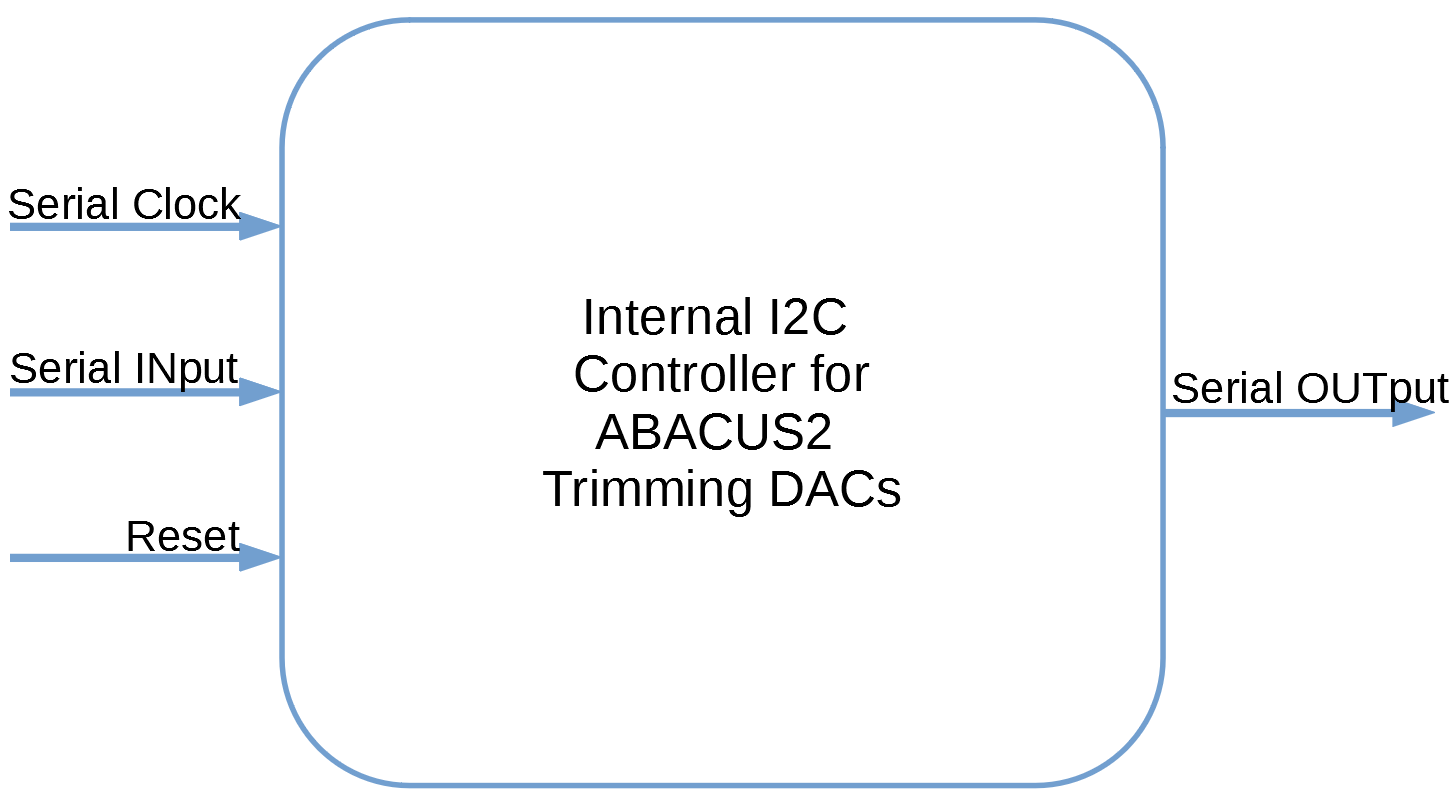
\includegraphics[width=0.4\linewidth]{IMG/ch4/INTERNALDAC}
	\caption{test bench}
	\label{fig:internaldac}
\end{figure}
\noindent The 2x24 threshold fine tuning DACs are controlled by 48 5-bits registers. These registers can be independently
loaded and read-out via a serial interface protocol based on 16-bits words. The commands are send via a Serial
INput pin (SIN) and the data are read-out on a Serial OUTput pin (SOUT). The two serial streams are
synchronous to the CLK clock input and are sampled on the clock rising edge.
The write operations are performed according to the following sequence:
\begin{itemize}
	\item Send start sequence : hex A5A5
	\item Send write command : 11a13...a8d7...d0
\end{itemize}

\begin{figure}[H]
	\centering
	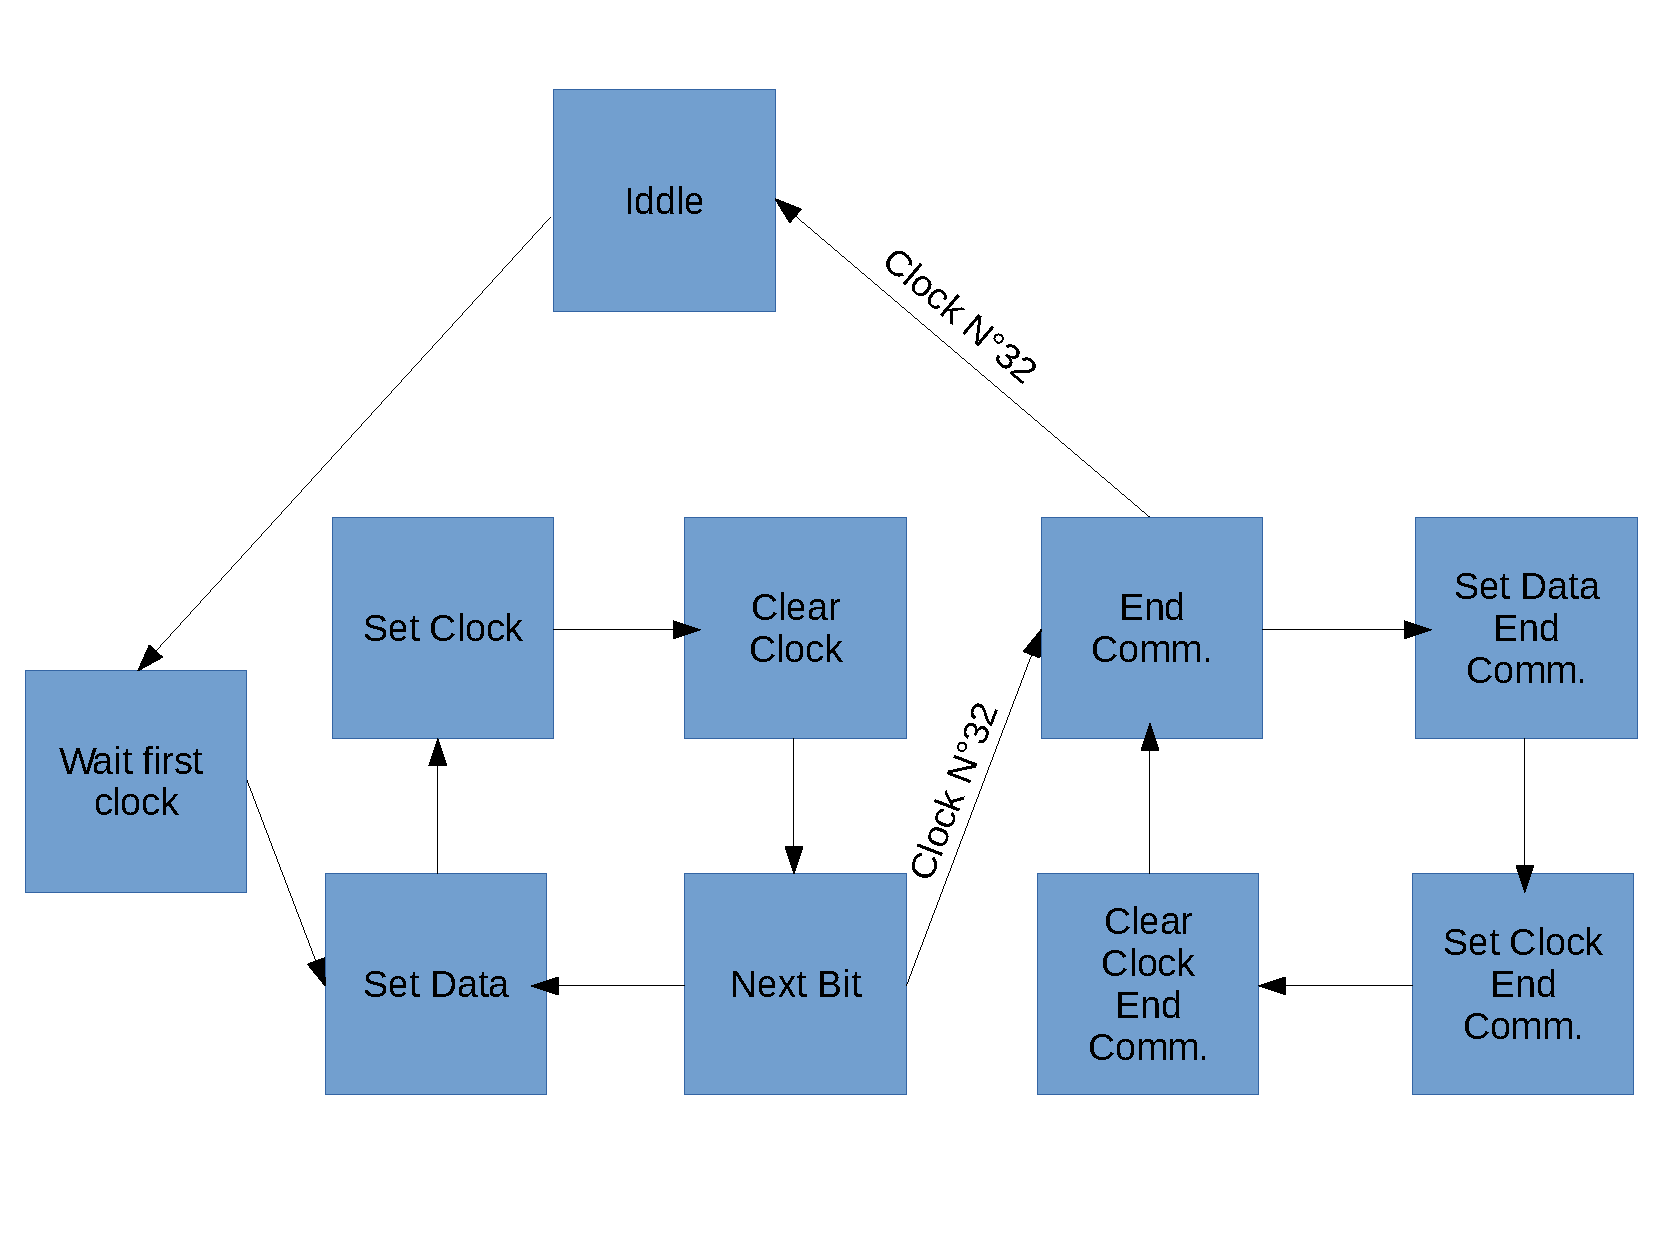
\includegraphics[width=0.7\linewidth]{IMG/ch4/FSM}
	\caption{test bench}
	\label{fig:fsm}
\end{figure}

\subsection{Latching counters}

\subsection{Timestamp generator}

\section{Simulations}

\subsection{Internal DAC simulation}

\subsection{Latching counters simulation}

\subsection{Timestamp generator simulation}

\section{Hardware devices}\label{hardware}

\begin{figure}[H]
	\centering
	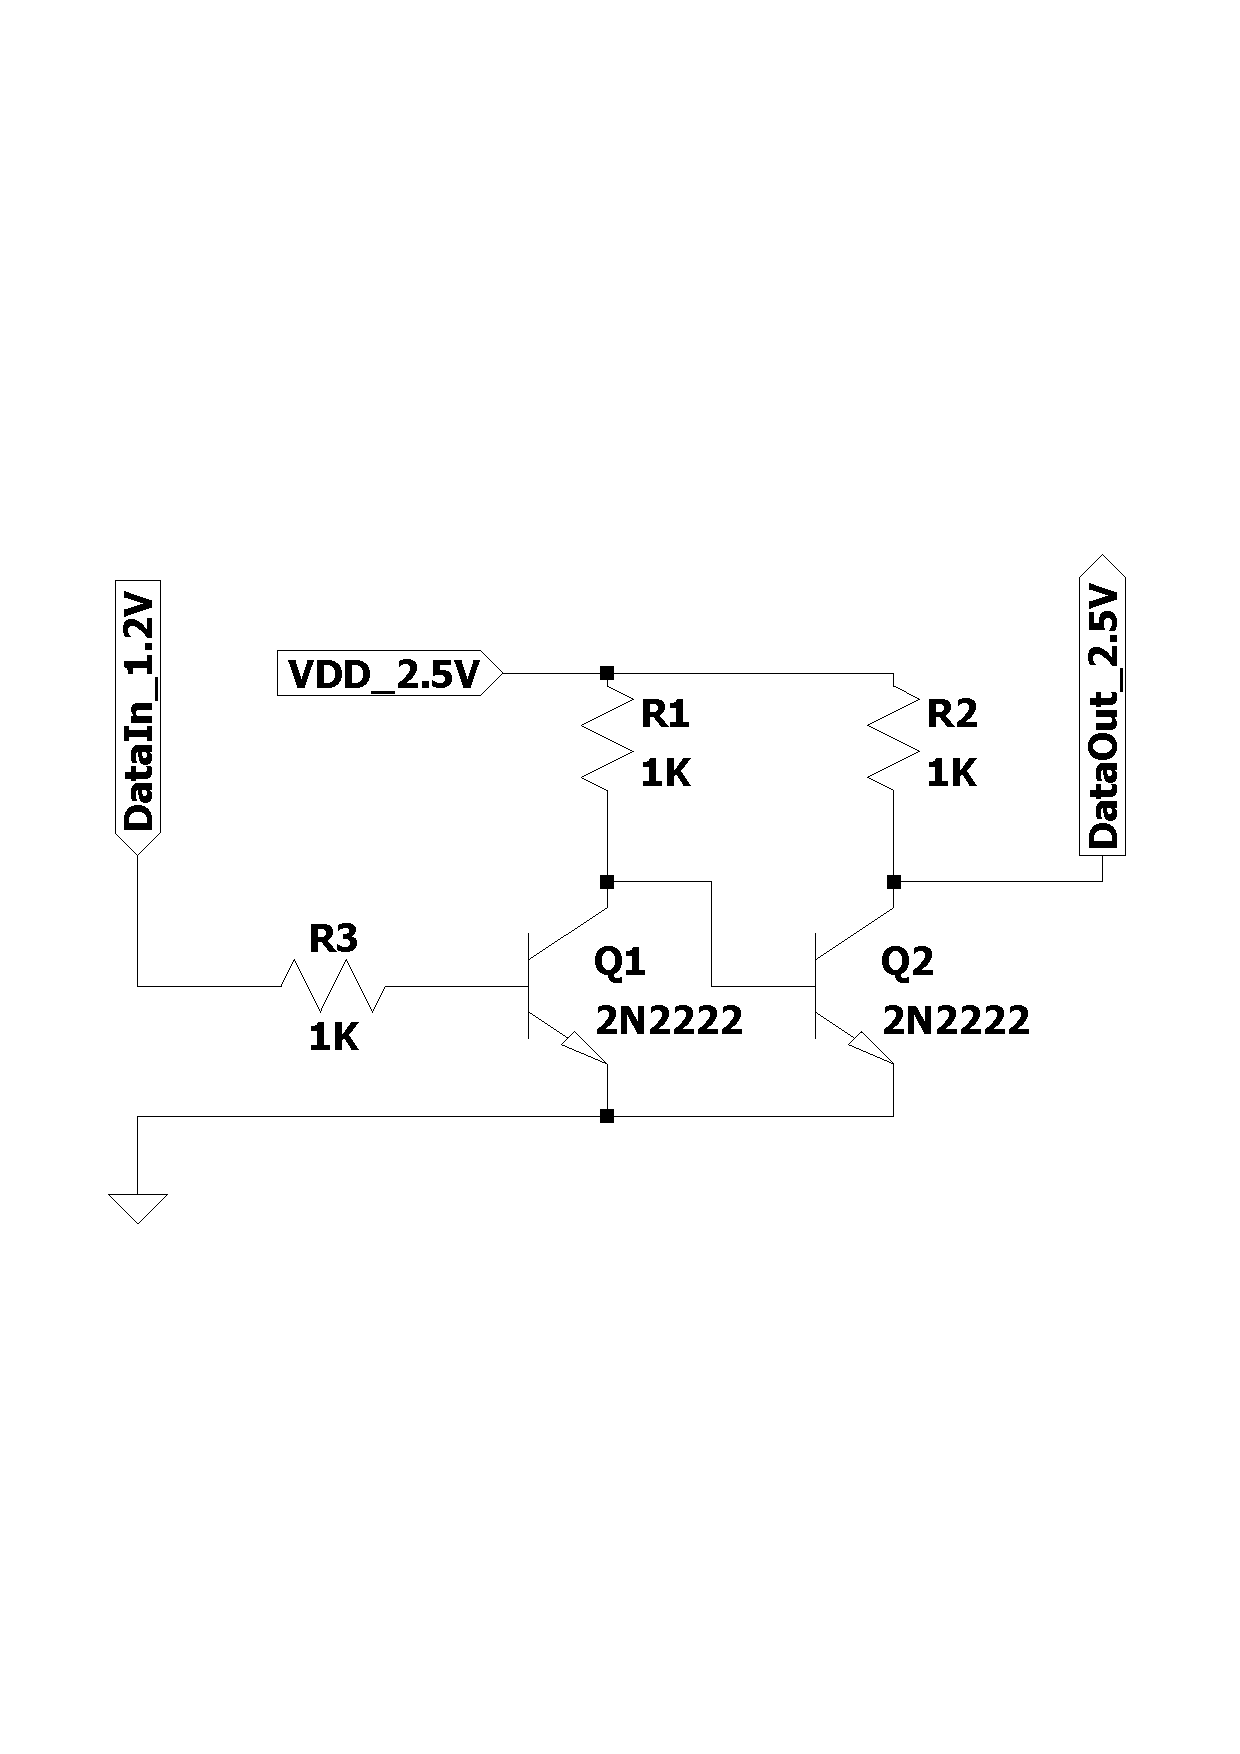
\includegraphics[width=0.7\linewidth]{IMG/ch4/DIAGRAM}
	\caption{test bench}
	\label{fig:diagram}
\end{figure}


\section{Test Bench}\label{testbench}
\begin{figure}[H]
	\centering
	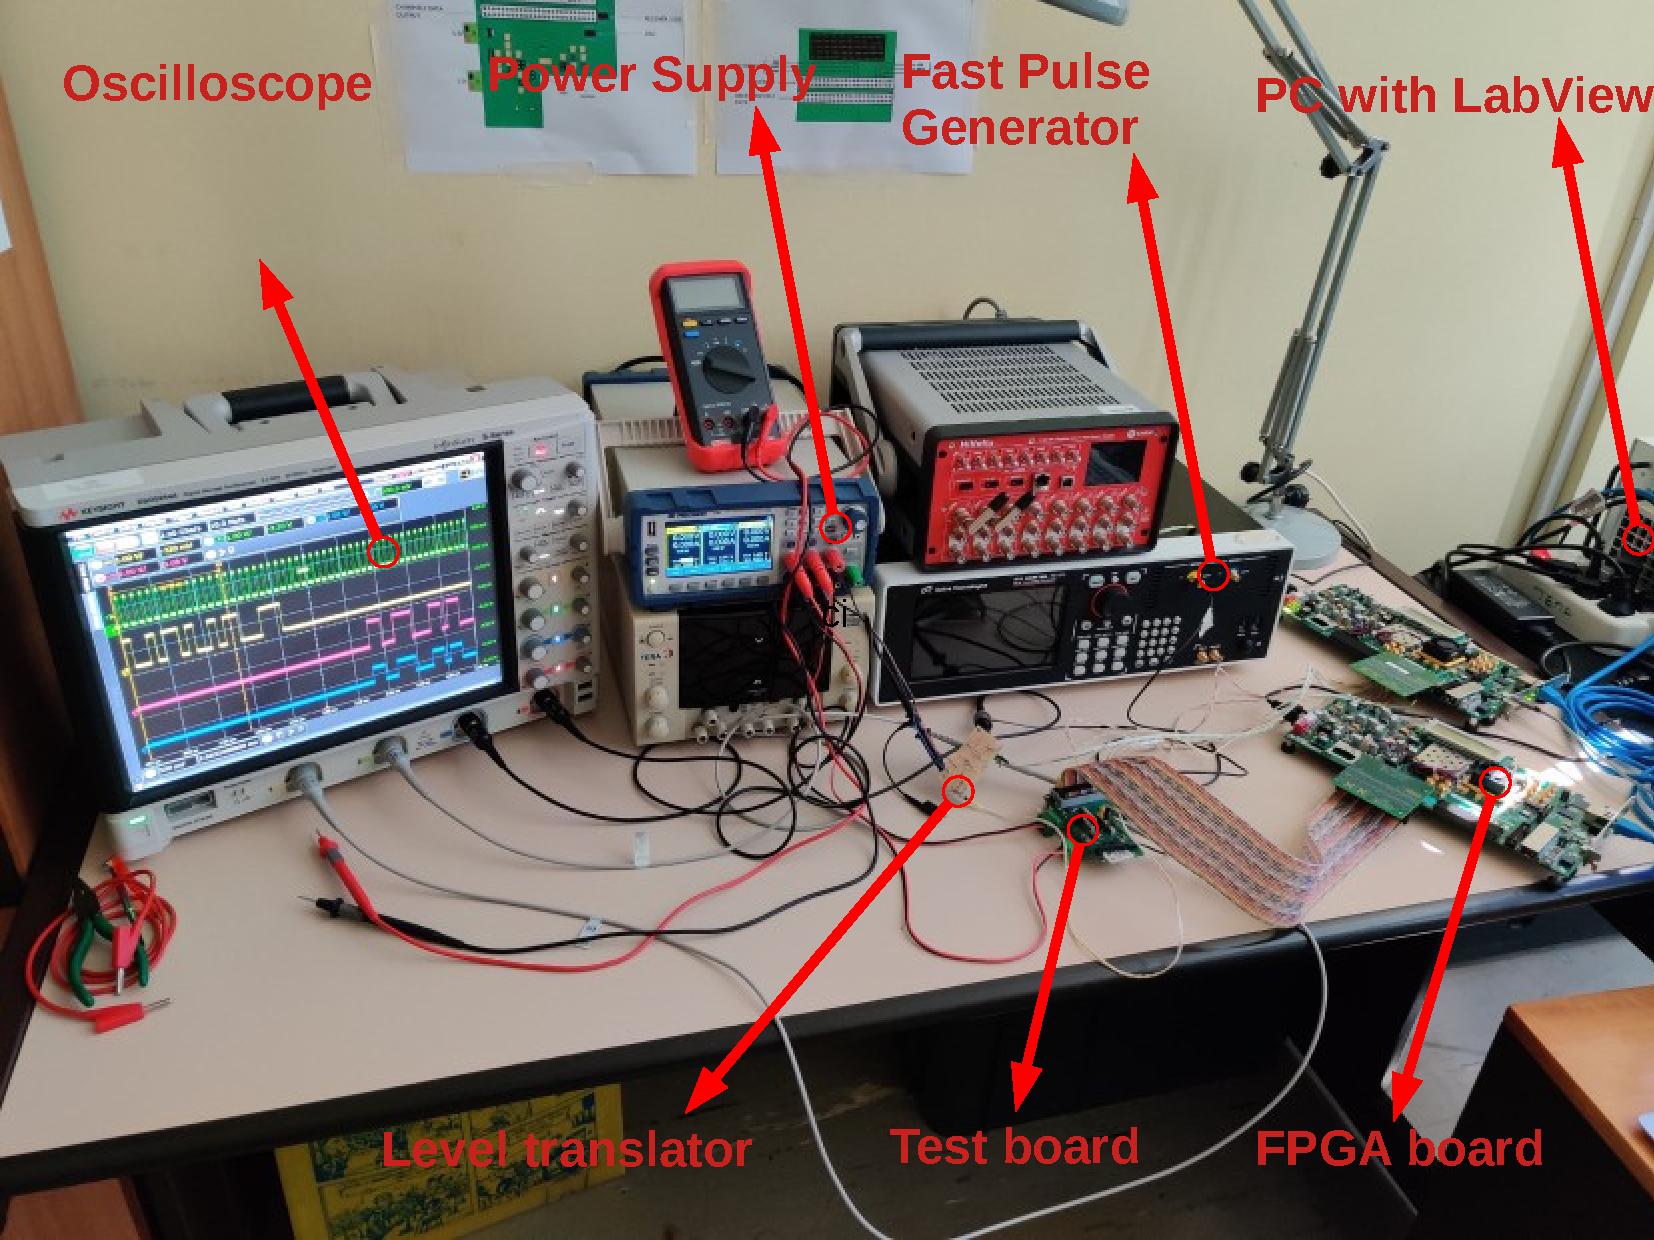
\includegraphics[width=0.7\linewidth]{IMG/ch4/TESTBENCH}
	\caption{test bench}
	\label{fig:testbench}
\end{figure}

\section{Test board}\label{testboard}
\begin{figure}[H]
	\centering
	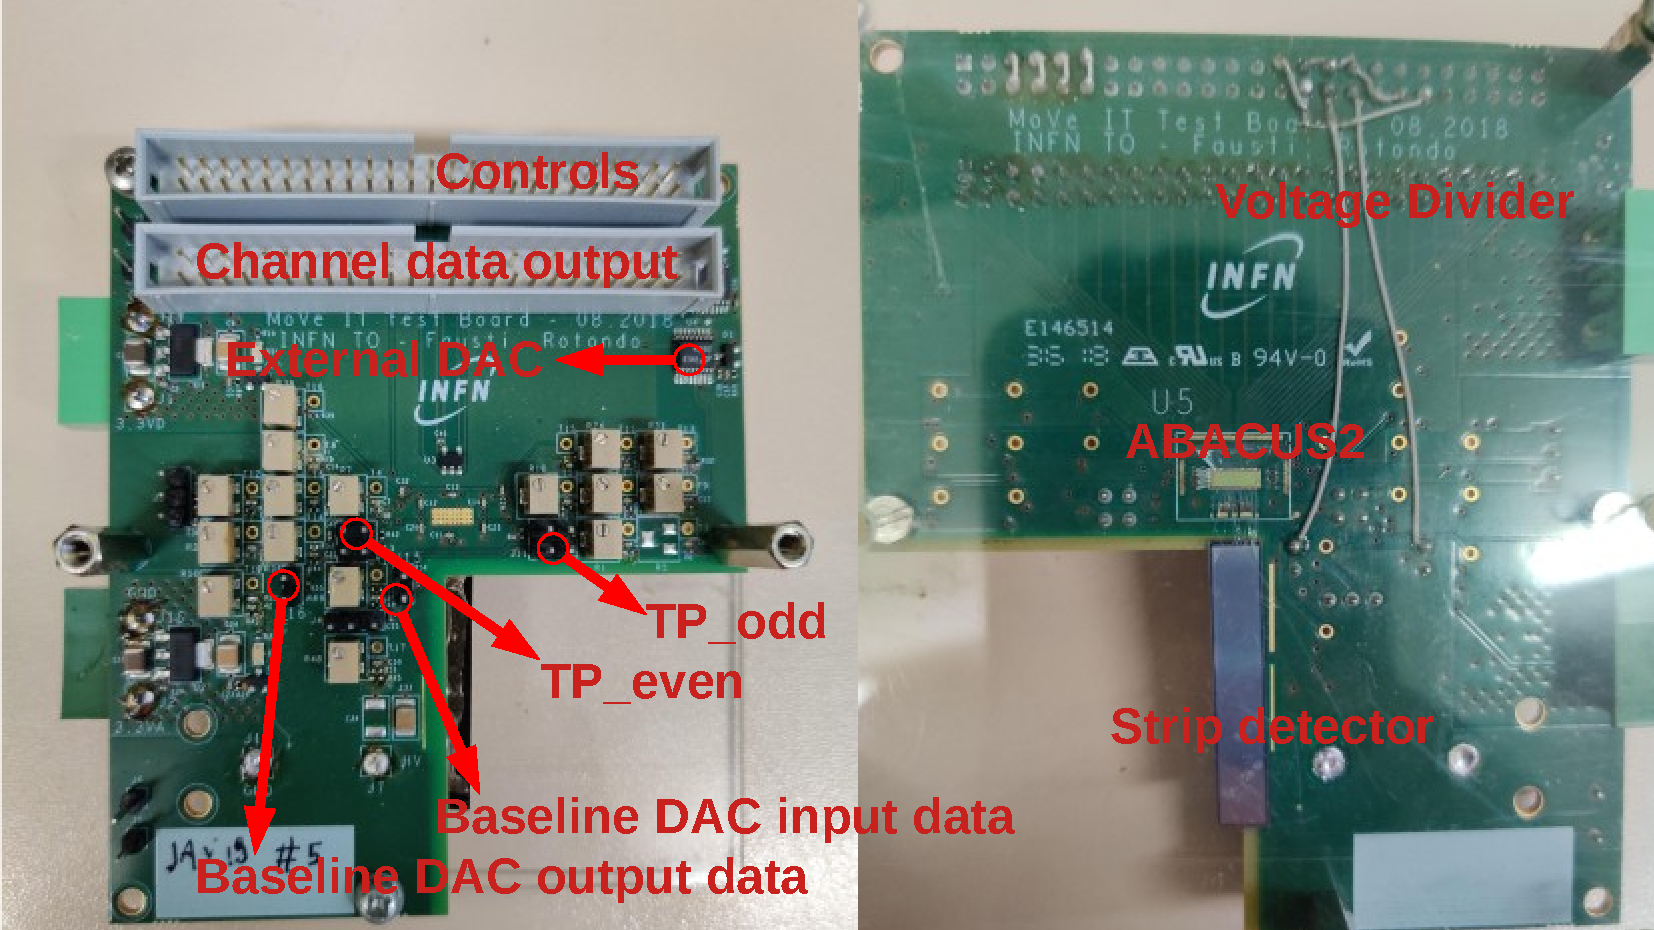
\includegraphics[width=0.7\linewidth]{IMG/ch4/TESTBOARD}
	\caption{test board}
	\label{fig:testboard}
\end{figure}

\section{Esa-Abacus}
